\section{Introduction}
\label{sec:intro}

\begin{figure}
    \centering
    \makebox[\textwidth][c]{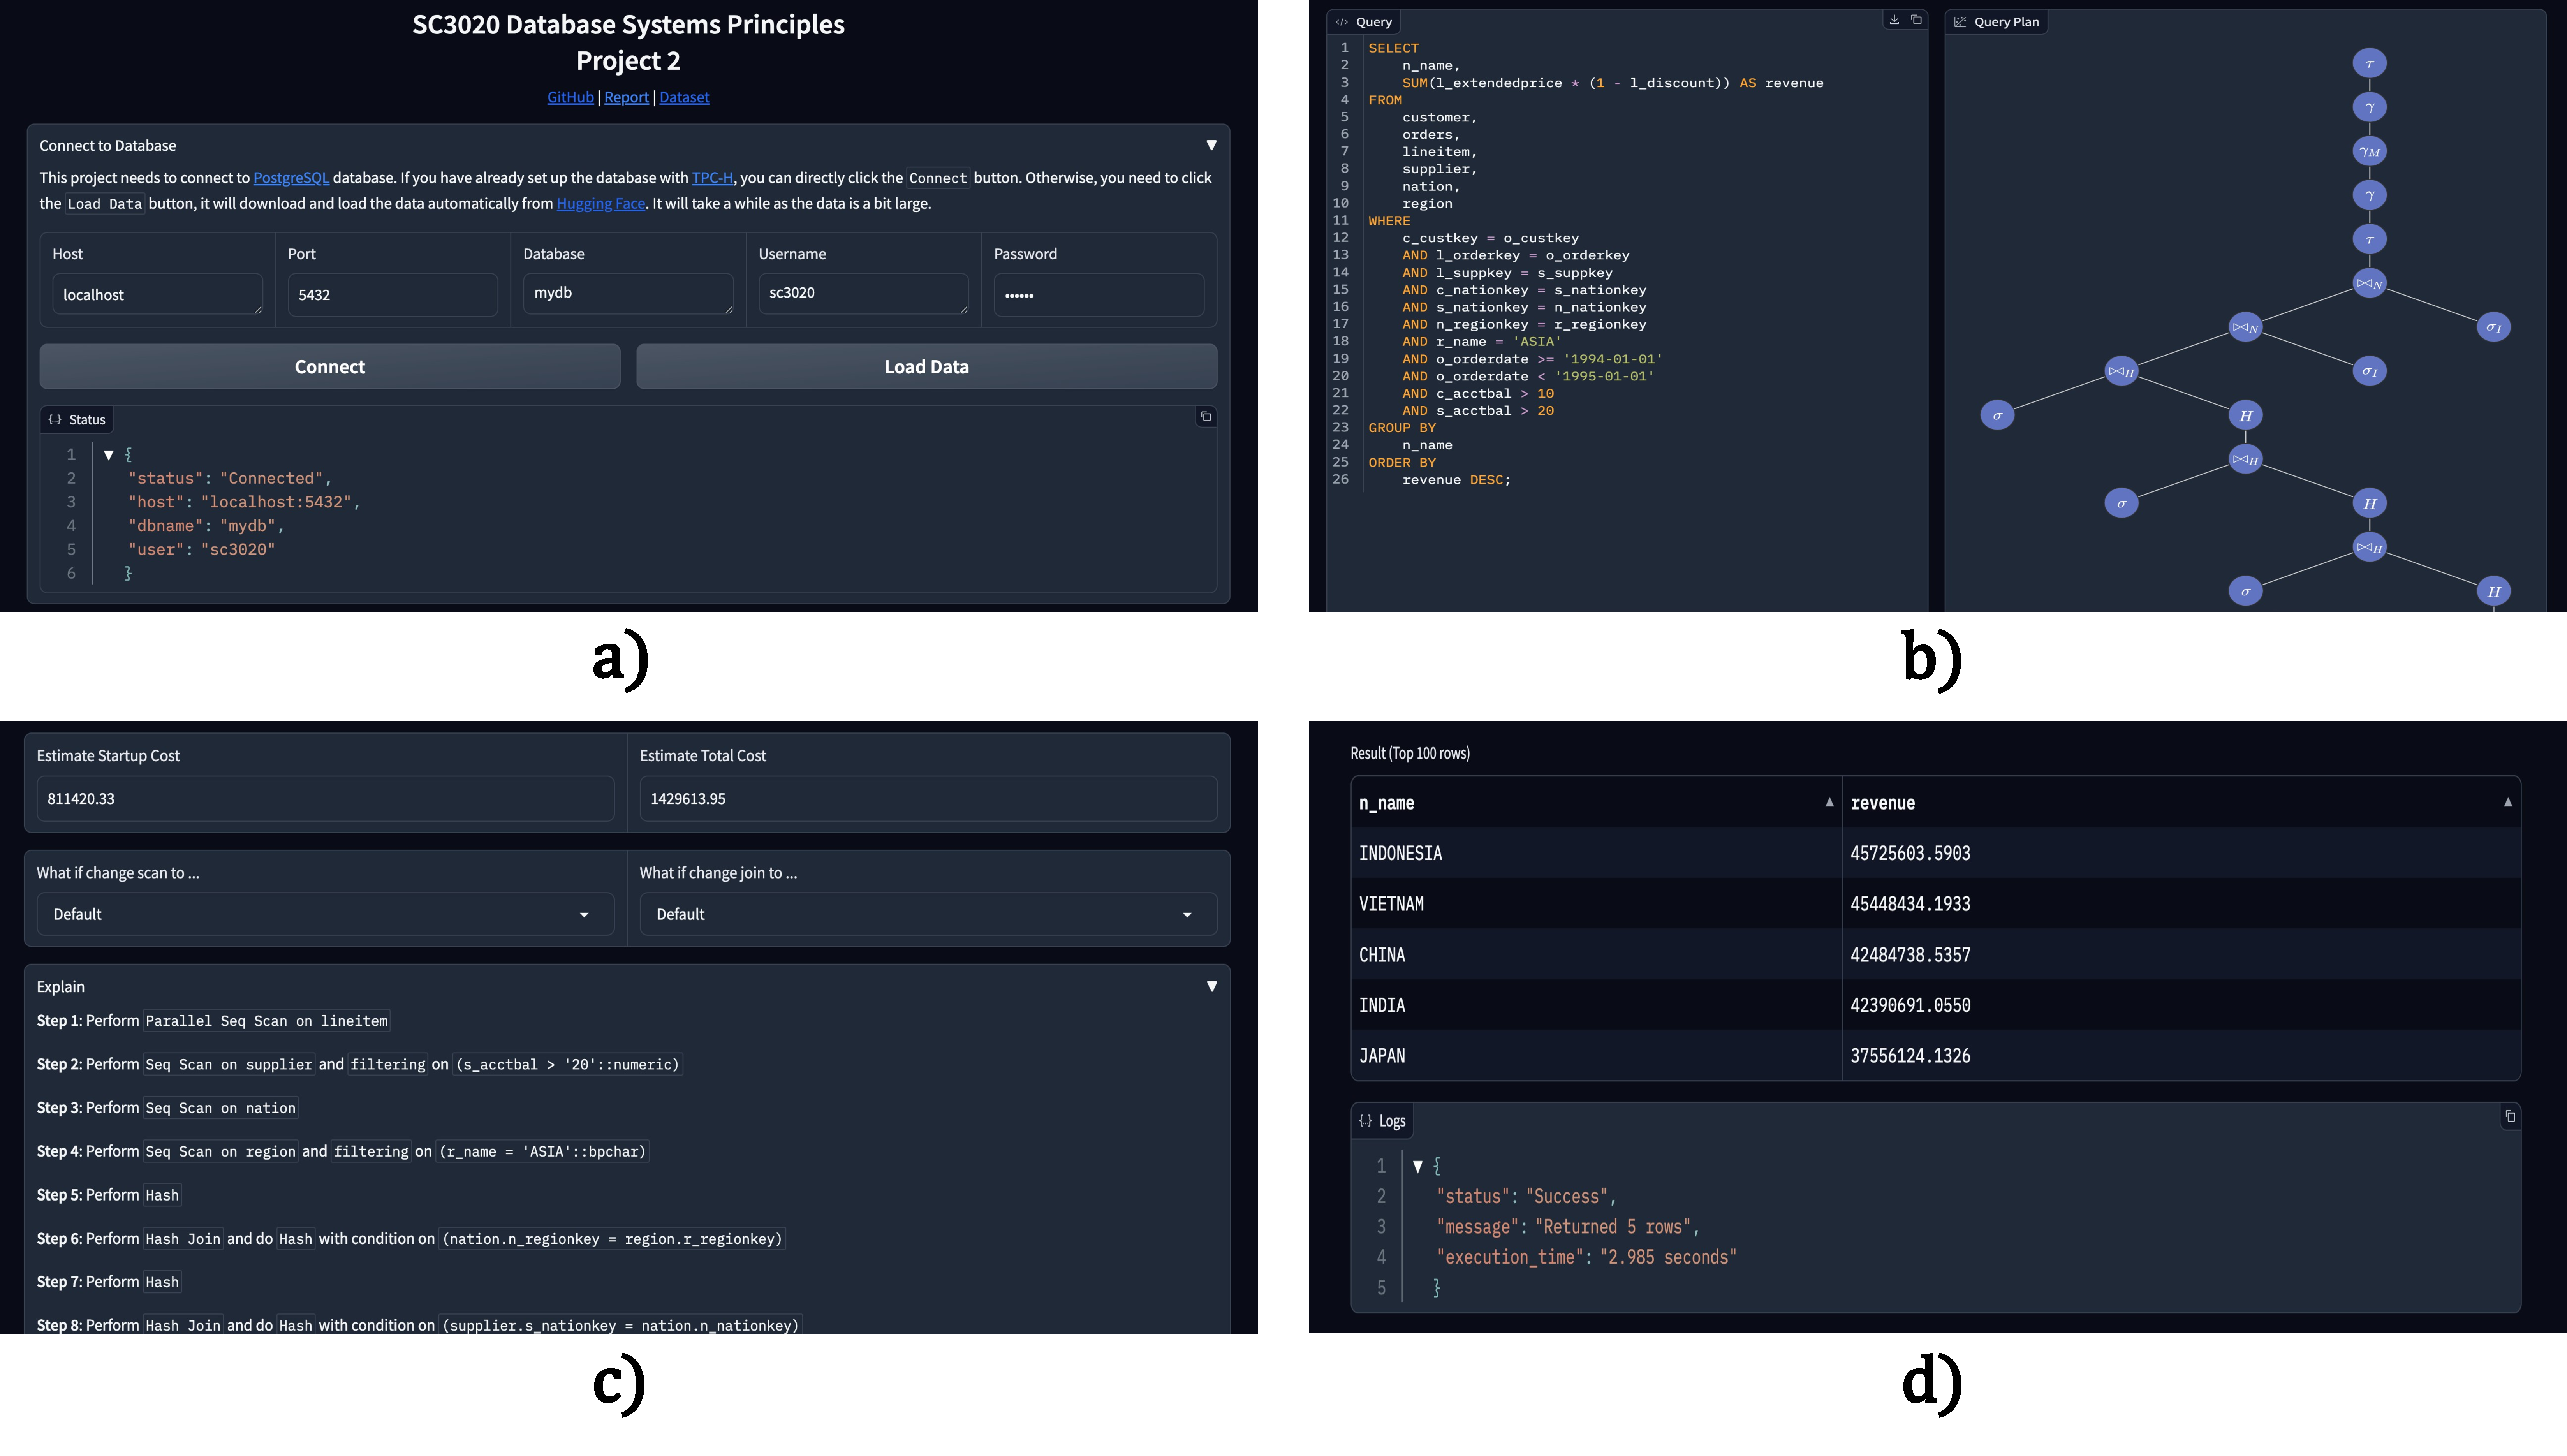
\includegraphics[width=1.3\linewidth]{figures/overview.pdf}}
    \caption{An overview of our designed UI. \textbf{a)} We provide an interface to allow you to connect to the SQL server running in backend with your own config. By clicking Load Data, we will fetch the data we use and create data in your selected db. \textbf{b)} We allow you to write query and visualize an interactive query plan. \textbf{c)} We estimated startup cost and total cost with explanation. You can change the config with the dropdown. \textbf{d)} We also allow you to execute the SQL query and log the result.}
    \label{fig:Overview}
\end{figure}

In real-world applications, writing SQL to retrieve information from a DBMS has become a routine task. However, since I/O costs significantly impact query performance, it is often necessary to optimize the query plan based on specific requirements. In PostgreSQL~\citep{postgres_github}, the query execution plan (QEP) is generated from a large number of alternative query plans (AQPs). Therefore, it is essential to provide the following capabilities:

\begin{itemize} 
    \item Retrieve and visualize the QEP for a given SQL query 
    \item Support ``what-if'' queries on the QEP 
    \item Retrieve the estimated cost of the AQPs 
\end{itemize}

To achieve these objectives, we developed a user interface (UI) that allows users to interactively modify their QEPs based on their needs. The functionalities of our application are demonstrated in~\cref{fig:Overview}. The application enables users to connect to an existing database they have created and creates tables from the prepared data fetched from the Internet. Users can then write SQL queries and visualize the corresponding query plans. Additionally, they can view the estimated costs, modify the types of scan or join methods, and optimize the plan based on their requirements. Once satisfied with the cost, users can execute the commands, log the results, and evaluate the performance.

The remainder of this report is structured as follows:

\begin{itemize} 
    \item An overview of the pipeline and the structure of our application
    \item A detailed explanation of the algorithms
    \item Case studies demonstrating the application
\end{itemize}

